\documentclass[a4paper]{article}

% \usepackage[english]{babel}
% \usepackage[utf8]{inputenc}
% \usepackage{amsmath}
% \usepackage{graphicx}
% \usepackage[colorinlistoftodos]{todonotes}
% \documentclass[a4paper]{article}

\usepackage[english]{babel}
\usepackage[utf8]{inputenc}
\usepackage{amsmath}
\usepackage{graphicx}
\usepackage{parskip}
\usepackage{amssymb}

\newcommand{\coinblack}{\blacksquare}
\newcommand{\coinwhite}{\square}
\newcommand{\coinempty}{-}

\title{ECE457a Assignment 1}

\author{Lucas Wojciechowksi, Ariel Weingarten, Alexander Maguire, Austin Dobrik, Dane Carr}

\date{\today}

\begin{document}
\maketitle

\section{Question 1}

\subsection{Part A}

The game board consists of 7 squares, indexed from 0 to 6.

We can define every state within the game as a 7-tuple containing
\begin{itemize}
\item 3 black coins, denoted $\coinblack$
\item 2 white coins, denoted $\coinwhite$
\item 2 emptys, denoted $\coinempty$
\end{itemize}
The inital state is $s_0 = (\coinempty \coinempty \coinblack \coinwhite \coinblack \coinwhite \coinblack)$

Coins are moved as adjacent pairs. We define a pair of coins as $p_i$, where $i$ is the lowest-indexed square on which the coins rest. In the initial state, the first pair of coins is $p_2$.

Empty squares on the board always exist as a single adjacent pair, which we will also define by its lowest-indexed square. On the initial game board, the empty pair is at $p_0$.

Lets define a function, $\text{empty\_pair}(s)$ which, given a state $s$, returns the empty pair on the board. For example. $\text{empty\_pair}(s_0) = p_0$.

In any game state, $s$, the valid pairs are
$$\{p_i | i \in [0, 5] \backslash [\text{empty\_pair}(s) - 1, \text{empty\_pair}(s) + 1]\}$$
Each of these pairs corresponds with exactly one valid move
$$p_i \rightarrow \text{empty\_pair}(s)$$



\subsection{Part B}

\subsubsection{Breadth First Search}
\begin{center}
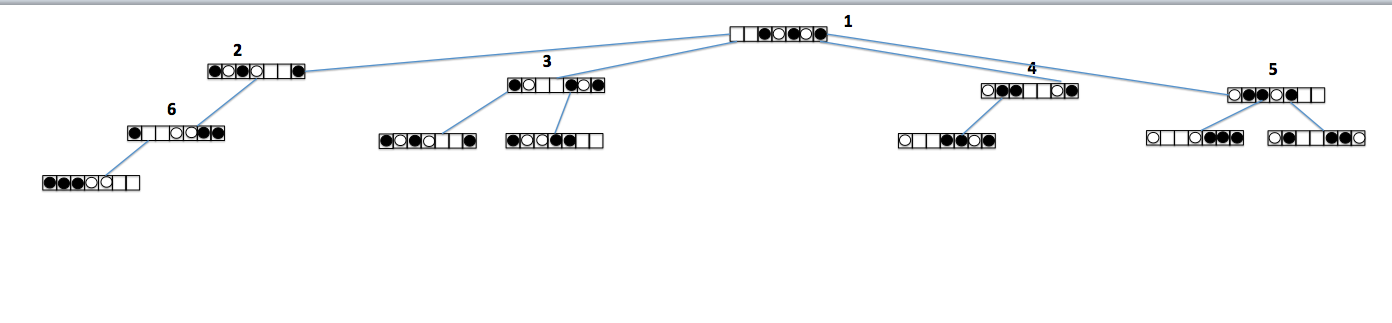
\includegraphics[width=1\textwidth]{BFS.png}
\end{center}

\subsubsection{Depth First Search (with depth limit of 3)}
\begin{center}
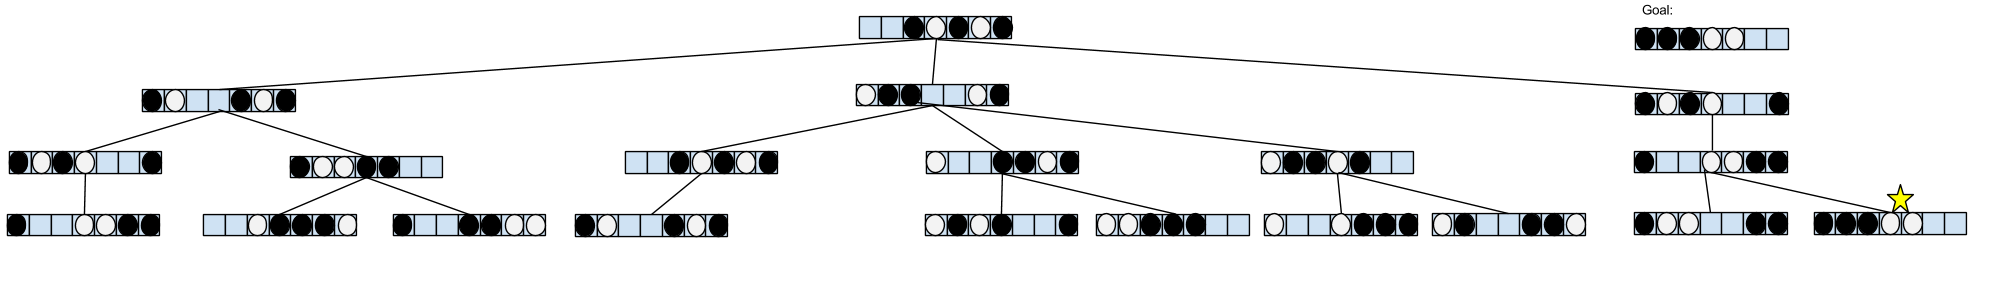
\includegraphics[width=1\textwidth]{DFS.png}
\end{center}


\subsubsection{Hill Climbing Search}
We used a simple and intuitive heuristic, where the value of each node is the number of squares that have the same coin as the goal state.
For example, if the goal state is $s_f = (\coinblack \coinblack \coinblack \coinwhite \coinwhite \coinempty \coinempty)$ then $s_0 = (\coinempty \coinempty \coinblack \coinwhite \coinblack \coinwhite \coinblack)$ has value 2.
\begin{center}
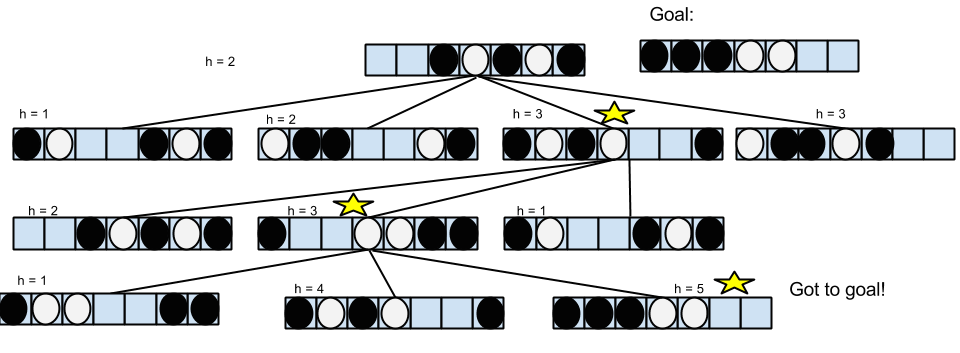
\includegraphics[width=1\textwidth]{HillClimbing.png}
\end{center}

\subsubsection{Best First Search (using heuristic developed in previous answer}
\begin{center}
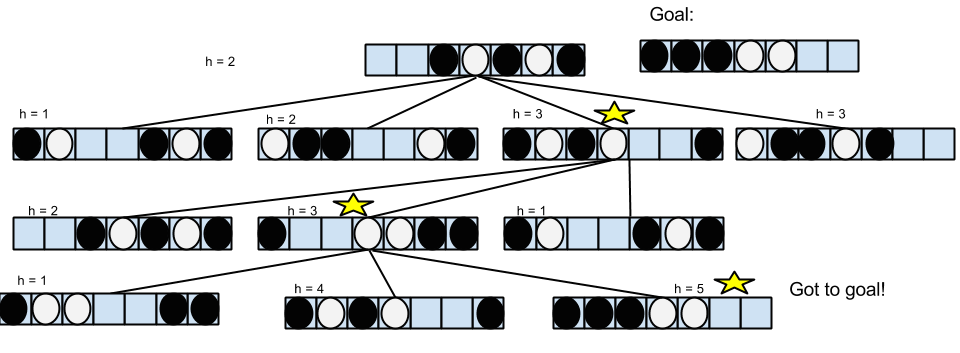
\includegraphics[width=1\textwidth]{BestFirst.png}
\end{center}

\subsubsection{Compare the performance of the above search strategies in terms of the number of nodes generated}
Breadth-first search generated 15 nodes before finding the solution, depth-first search generated 20, and hill climbing and best first generated 11.
Hill climbing and best first search followed the exact same path in this case, so their performance was the same.  However it may be different with a 
different heuristic or a different initial state. Note that the depth limit of 3 on depth first search forced the search to generate more nodes.  If it 
had been allowed to go to a depth of 4, depth-first search would have found the solution after only 6 nodes.

In this case, hill climbing and best first search are tied for best performance.

\section{Question 2}

% Insert picture of the MIN MAX tree from assignment


\subsection{Part A}
The root node minimax value is 8.
\begin{center}
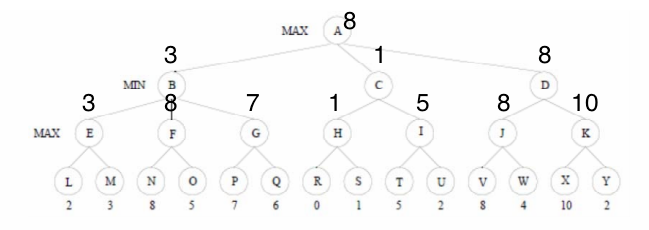
\includegraphics[width=1\textwidth]{a1q2a.png}
\end{center}

\subsection{Part B}
Max should choose node D.

\subsection{Part C}
Nodes {O, Q, U, Y} are not visited when $\alpha$-$\beta$ pruning is used.

\subsection{Part D}
Swap B and D, giving a final order of {D C B} on the second level of the tree.
This results in ten nodes being pruned: {Y, I, T, U, F, N, O, G, P, Q}.


\end{document}